% Options for packages loaded elsewhere
\PassOptionsToPackage{unicode}{hyperref}
\PassOptionsToPackage{hyphens}{url}
%
\documentclass[
  ignorenonframetext,
]{beamer}
\usepackage{pgfpages}
\setbeamertemplate{caption}[numbered]
\setbeamertemplate{caption label separator}{: }
\setbeamercolor{caption name}{fg=normal text.fg}
\beamertemplatenavigationsymbolsempty
% Prevent slide breaks in the middle of a paragraph
\widowpenalties 1 10000
\raggedbottom
\setbeamertemplate{part page}{
  \centering
  \begin{beamercolorbox}[sep=16pt,center]{part title}
    \usebeamerfont{part title}\insertpart\par
  \end{beamercolorbox}
}
\setbeamertemplate{section page}{
  \centering
  \begin{beamercolorbox}[sep=12pt,center]{part title}
    \usebeamerfont{section title}\insertsection\par
  \end{beamercolorbox}
}
\setbeamertemplate{subsection page}{
  \centering
  \begin{beamercolorbox}[sep=8pt,center]{part title}
    \usebeamerfont{subsection title}\insertsubsection\par
  \end{beamercolorbox}
}
\AtBeginPart{
  \frame{\partpage}
}
\AtBeginSection{
  \ifbibliography
  \else
    \frame{\sectionpage}
  \fi
}
\AtBeginSubsection{
  \frame{\subsectionpage}
}
\usepackage{amsmath,amssymb}
\usepackage{iftex}
\ifPDFTeX
  \usepackage[T1]{fontenc}
  \usepackage[utf8]{inputenc}
  \usepackage{textcomp} % provide euro and other symbols
\else % if luatex or xetex
  \usepackage{unicode-math} % this also loads fontspec
  \defaultfontfeatures{Scale=MatchLowercase}
  \defaultfontfeatures[\rmfamily]{Ligatures=TeX,Scale=1}
\fi
\usepackage{lmodern}
\ifPDFTeX\else
  % xetex/luatex font selection
\fi
% Use upquote if available, for straight quotes in verbatim environments
\IfFileExists{upquote.sty}{\usepackage{upquote}}{}
\IfFileExists{microtype.sty}{% use microtype if available
  \usepackage[]{microtype}
  \UseMicrotypeSet[protrusion]{basicmath} % disable protrusion for tt fonts
}{}
\makeatletter
\@ifundefined{KOMAClassName}{% if non-KOMA class
  \IfFileExists{parskip.sty}{%
    \usepackage{parskip}
  }{% else
    \setlength{\parindent}{0pt}
    \setlength{\parskip}{6pt plus 2pt minus 1pt}}
}{% if KOMA class
  \KOMAoptions{parskip=half}}
\makeatother
\usepackage{xcolor}
\newif\ifbibliography
\usepackage{color}
\usepackage{fancyvrb}
\newcommand{\VerbBar}{|}
\newcommand{\VERB}{\Verb[commandchars=\\\{\}]}
\DefineVerbatimEnvironment{Highlighting}{Verbatim}{commandchars=\\\{\}}
% Add ',fontsize=\small' for more characters per line
\usepackage{framed}
\definecolor{shadecolor}{RGB}{248,248,248}
\newenvironment{Shaded}{\begin{snugshade}}{\end{snugshade}}
\newcommand{\AlertTok}[1]{\textcolor[rgb]{0.94,0.16,0.16}{#1}}
\newcommand{\AnnotationTok}[1]{\textcolor[rgb]{0.56,0.35,0.01}{\textbf{\textit{#1}}}}
\newcommand{\AttributeTok}[1]{\textcolor[rgb]{0.13,0.29,0.53}{#1}}
\newcommand{\BaseNTok}[1]{\textcolor[rgb]{0.00,0.00,0.81}{#1}}
\newcommand{\BuiltInTok}[1]{#1}
\newcommand{\CharTok}[1]{\textcolor[rgb]{0.31,0.60,0.02}{#1}}
\newcommand{\CommentTok}[1]{\textcolor[rgb]{0.56,0.35,0.01}{\textit{#1}}}
\newcommand{\CommentVarTok}[1]{\textcolor[rgb]{0.56,0.35,0.01}{\textbf{\textit{#1}}}}
\newcommand{\ConstantTok}[1]{\textcolor[rgb]{0.56,0.35,0.01}{#1}}
\newcommand{\ControlFlowTok}[1]{\textcolor[rgb]{0.13,0.29,0.53}{\textbf{#1}}}
\newcommand{\DataTypeTok}[1]{\textcolor[rgb]{0.13,0.29,0.53}{#1}}
\newcommand{\DecValTok}[1]{\textcolor[rgb]{0.00,0.00,0.81}{#1}}
\newcommand{\DocumentationTok}[1]{\textcolor[rgb]{0.56,0.35,0.01}{\textbf{\textit{#1}}}}
\newcommand{\ErrorTok}[1]{\textcolor[rgb]{0.64,0.00,0.00}{\textbf{#1}}}
\newcommand{\ExtensionTok}[1]{#1}
\newcommand{\FloatTok}[1]{\textcolor[rgb]{0.00,0.00,0.81}{#1}}
\newcommand{\FunctionTok}[1]{\textcolor[rgb]{0.13,0.29,0.53}{\textbf{#1}}}
\newcommand{\ImportTok}[1]{#1}
\newcommand{\InformationTok}[1]{\textcolor[rgb]{0.56,0.35,0.01}{\textbf{\textit{#1}}}}
\newcommand{\KeywordTok}[1]{\textcolor[rgb]{0.13,0.29,0.53}{\textbf{#1}}}
\newcommand{\NormalTok}[1]{#1}
\newcommand{\OperatorTok}[1]{\textcolor[rgb]{0.81,0.36,0.00}{\textbf{#1}}}
\newcommand{\OtherTok}[1]{\textcolor[rgb]{0.56,0.35,0.01}{#1}}
\newcommand{\PreprocessorTok}[1]{\textcolor[rgb]{0.56,0.35,0.01}{\textit{#1}}}
\newcommand{\RegionMarkerTok}[1]{#1}
\newcommand{\SpecialCharTok}[1]{\textcolor[rgb]{0.81,0.36,0.00}{\textbf{#1}}}
\newcommand{\SpecialStringTok}[1]{\textcolor[rgb]{0.31,0.60,0.02}{#1}}
\newcommand{\StringTok}[1]{\textcolor[rgb]{0.31,0.60,0.02}{#1}}
\newcommand{\VariableTok}[1]{\textcolor[rgb]{0.00,0.00,0.00}{#1}}
\newcommand{\VerbatimStringTok}[1]{\textcolor[rgb]{0.31,0.60,0.02}{#1}}
\newcommand{\WarningTok}[1]{\textcolor[rgb]{0.56,0.35,0.01}{\textbf{\textit{#1}}}}
\usepackage{graphicx}
\makeatletter
\def\maxwidth{\ifdim\Gin@nat@width>\linewidth\linewidth\else\Gin@nat@width\fi}
\def\maxheight{\ifdim\Gin@nat@height>\textheight\textheight\else\Gin@nat@height\fi}
\makeatother
% Scale images if necessary, so that they will not overflow the page
% margins by default, and it is still possible to overwrite the defaults
% using explicit options in \includegraphics[width, height, ...]{}
\setkeys{Gin}{width=\maxwidth,height=\maxheight,keepaspectratio}
% Set default figure placement to htbp
\makeatletter
\def\fps@figure{htbp}
\makeatother
\setlength{\emergencystretch}{3em} % prevent overfull lines
\providecommand{\tightlist}{%
  \setlength{\itemsep}{0pt}\setlength{\parskip}{0pt}}
\setcounter{secnumdepth}{-\maxdimen} % remove section numbering
\ifLuaTeX
  \usepackage{selnolig}  % disable illegal ligatures
\fi
\IfFileExists{bookmark.sty}{\usepackage{bookmark}}{\usepackage{hyperref}}
\IfFileExists{xurl.sty}{\usepackage{xurl}}{} % add URL line breaks if available
\urlstyle{same}
\hypersetup{
  pdftitle={TMA4315 Generalized linear models H2018},
  pdfauthor={Mette Langaas, Department of Mathematical Sciences, NTNU -- with contributions from Ingeborg Hem},
  hidelinks,
  pdfcreator={LaTeX via pandoc}}

\title{TMA4315 Generalized linear models H2018}
\subtitle{Module 4: Count and continuous positive response data (Poisson
and gamma regression)}
\author{Mette Langaas, Department of Mathematical Sciences, NTNU -- with
contributions from Ingeborg Hem}
\date{27.09.2018 and 04.10.2018 {[}PL{]}, 28.09.2018 and 05.10.2018
{[}IL{]}}

\begin{document}
\frame{\titlepage}

\begin{frame}
(Latest changes: 06.10: solutions added. 01.10: small changes for second
week. 27.09: added one Problem for ILw1, moved stuff to w2, added a few
dimensions to score test.)
\end{frame}

\begin{frame}{Overview}
\protect\hypertarget{overview}{}
\begin{block}{Learning material}
\protect\hypertarget{learning-material}{}
\begin{itemize}
\tightlist
\item
  Textbook: Fahrmeir et al (2013): Chapter 5.2, 5.3.
\item
  \href{https://www.math.ntnu.no/emner/TMA4315/2018h/TMA4315M4H20180927.pdf}{Classnotes
  27.09.2018}
\item
  \href{https://www.math.ntnu.no/emner/TMA4315/2018h/TMA4315M4H20181004.pdf}{Classnotes
  04.10.2018}
\end{itemize}
\end{block}
\end{frame}

\begin{frame}
\begin{block}{Topics}
\protect\hypertarget{topics}{}
\begin{block}{\protect\hyperlink{firstweek}{First week}}
\protect\hypertarget{first-week}{}
\begin{itemize}
\tightlist
\item
  examples of count data
\item
  the Poisson distribution
\item
  regression with count data
\item
  Poisson regression with log-link
\item
  parameter estimation (ML): log-likelhood, score vector, information
  matrix to give iterative calculations
\item
  asymptotic MLE properties
\item
  confidence intervals and hypothesis tests (Wald, score and LRT)
\end{itemize}

Jump to \protect\hyperlink{interactivew1}{interactive (week 1)}
\end{block}
\end{block}
\end{frame}

\begin{frame}
\begin{block}{\protect\hyperlink{secondweek}{Second week}}
\protect\hypertarget{second-week}{}
\begin{itemize}
\item
  Count data with Poisson regression (continued)
\item
  deviance, model fit and model choice
\item
  overdispersion
\item
  rate models and offset
\item
  Modelling continuous response data: lognormal and gamma
\item
  the gamma distribution
\item
  the gamma GLM model
\item
  gamma likelihood and derivations thereof
\item
  dispersion parameter: scaled and unscaled deviance
\end{itemize}
\end{block}
\end{frame}

\begin{frame}
\textbf{ SECOND WEEK}
\end{frame}

\begin{frame}{Poisson regression for count data}
\protect\hypertarget{poisson-regression-for-count-data}{}
What did we do last week?

Examples --- GLM model --- loglikelihood, score function and Fisher
information matrix --- asympototic results for
\(\hat{\boldsymbol{\beta}}\) and Wald, score and LRT.
\end{frame}

\begin{frame}{Deviance}
\protect\hypertarget{deviance}{}
The deviance is the difference in model fit between 2 models. Three
models are helpful:

\begin{itemize}
\tightlist
\item
  \textbf{Null model}: model with only an intercept
\item
  \textbf{Candidate model:} The model that we are investigating. We
  maximize the likelihood and get \(\hat{\beta}\)
\item
  \textbf{Saturated model:} A model with a parameter for every
  \(\lambda_i\) by the observed count for observation \(i\).
\end{itemize}

Notation:

\(\hat{\lambda}_i = \hat{y}_i\): prediction for the candidate model for
observation \(i\) \(\tilde{\lambda}_i=y_i\): prediction for the
saturated model for observation \(i\)
\end{frame}

\begin{frame}{Model assessment and model choice: using the deviance}
\protect\hypertarget{model-assessment-and-model-choice-using-the-deviance}{}
The fit of the model can be assessed based on goodness of fit statistics
(and related tests) and by residual plots. Model choice can be made from
analysis of deviance, or by comparing the AIC for different models.
\end{frame}

\begin{frame}
\begin{block}{Deviance}
\protect\hypertarget{deviance-1}{}
The (log-) likelihood ratio between two models is

\[
\begin{aligned}
l(\bar{\bar{\theta}}) - l(\bar{\theta}) &=\sum_{i=1}^n [y_i \ln(\bar{\bar{y}}_i)-\bar{\bar{y}}_i-\ln(y!)] - \sum_{i=1}^n [y_i \ln(\bar{y}_i)-\bar{y}_i-\ln(y!)] \\
&= \sum_{i=1}^n [y_i \left(\ln(\bar{\bar{y}}_i) - \ln(\bar{y}_i) \right)-\bar{\bar{y}}_i-\bar{y}_i] \\
&= \sum_{i=1}^n [y_i \ln(\bar{\bar{y}}_i/\bar{y}_i)- (\bar{\bar{y}}_i-\bar{y}_i)] \\
\end{aligned}
\]

The Saturated Deviance is

\[
D = -2 l(\theta)=-2\sum_{i=1}^n [y_i \ln(y_i)-y_i-\ln(y!)] 
\]

because \(\hat{y}_i = y_i\) for this model
\end{block}
\end{frame}

\begin{frame}{Deviance test}
\protect\hypertarget{deviance-test}{}
\[
\begin{aligned}
D&=-2(\ln L(\text{candidate model})-\ln L(\text{saturated model})) \\
&=-2(l(\hat{\pi})-l(\tilde{\pi}))=
-2\sum_{j=1}^G(l_j(\hat{\pi}_j)-l_j(\tilde{\pi}_j))
\end{aligned}
\]
\end{frame}

\begin{frame}
\begin{block}{Likelihood Ratio Tests with Deviance}
\protect\hypertarget{likelihood-ratio-tests-with-deviance}{}
The likelihood ratio test can be performed using the difference between
two deviances:

\[
\begin{aligned}
LRT &= D_1 - D_2 =-2(l_1(\hat{\pi}_1)-l(\tilde{\pi})) - (-2(l_2(\hat{\pi}_2)-l(\tilde{\pi}))) \\
&=-2(l_1(\hat{\pi}_1)-l_2(\tilde{\pi}_2))
\end{aligned}
\]

This follows a \(\chi^2_p\) distribution with \(k\) equal to the
difference in number of parameters
\end{block}
\end{frame}

\begin{frame}
\begin{block}{Deviance test}
\protect\hypertarget{deviance-test-1}{}
We may use the deviance test presented in Module 3 to test if the model
under study is preferred compared to the saturated model.

\[ D=2 \sum_{i=1}^n [y_i\ln(\frac{y_i}{\hat{y}_i})-(y_i-\hat{y}_i)]\]

Remark: if \(\sum_{i=1}^n y_i=\sum_{i=1}^n \hat{y}_i\) then deviance
will be equal to \[ D=2 \sum_{i=1}^n y_i\ln(\frac{y_i}{\hat{y}_i})\]

The deviance statistic approximately follows a \(\chi^2_{n-p}\), at
least when the counts are not low.
\end{block}
\end{frame}

\begin{frame}
\begin{block}{Pearson test}
\protect\hypertarget{pearson-test}{}
The Pearson \(\chi^2\)-goodness of fit statistic is given as the sum of
the squared Pearson residuals

\[ X_P^2=\sum_{i=1}^n r_i^2=\sum_{i=1}^n  \frac{(y_j-\hat{y}_i)^2}{\hat{y}_i}\]
where \(\hat{y}_i=\hat{\lambda}_i=\exp({\bf x}_i^T\hat{\beta})\). The
Pearson \(\chi^2\) statistic is asymptotically equivalent to the
deviance statistic and thus is asymptotically \(\chi^2_{n-p}\) (proof:
do a Taylor series expansion of the deviance).
\end{block}
\end{frame}

\begin{frame}
\begin{block}{Remarks}
\protect\hypertarget{remarks}{}
The asymptotic distribution of both statistics (deviance and Pearson)
are questionable when there are many low counts. Agresti (1996, page
990) suggest analysing grouped data, for example by grouping by width in
the horseshoe crab example.

The Pearson statistic is also used for testing independence in
contingency tables - we will do that in Compulsory Exercise 2.
\end{block}
\end{frame}

\begin{frame}[fragile]
\begin{block}{Example: goodness of fit with female horseshoe crabs}
\protect\hypertarget{example-goodness-of-fit-with-female-horseshoe-crabs}{}
Comment on the analysis. Is this a good fit? What might a bad fit be due
to?

\begin{Shaded}
\begin{Highlighting}[]
\NormalTok{model3 }\OtherTok{=} \FunctionTok{glm}\NormalTok{(Sa }\SpecialCharTok{\textasciitilde{}}\NormalTok{ W }\SpecialCharTok{+}\NormalTok{ C, }\AttributeTok{family =} \FunctionTok{poisson}\NormalTok{(}\AttributeTok{link =}\NormalTok{ log), }\AttributeTok{data =}\NormalTok{ crab, }\AttributeTok{contrasts =} \FunctionTok{list}\NormalTok{(}\AttributeTok{C =} \StringTok{"contr.sum"}\NormalTok{))}
\CommentTok{\# summary(model3)}
\DecValTok{1} \SpecialCharTok{{-}} \FunctionTok{pchisq}\NormalTok{(model3}\SpecialCharTok{$}\NormalTok{deviance, model3}\SpecialCharTok{$}\NormalTok{df.residual)}
\NormalTok{Xp }\OtherTok{=} \FunctionTok{sum}\NormalTok{(}\FunctionTok{residuals}\NormalTok{(model3, }\AttributeTok{type =} \StringTok{"pearson"}\NormalTok{)}\SpecialCharTok{\^{}}\DecValTok{2}\NormalTok{)}
\NormalTok{Xp}
\DecValTok{1} \SpecialCharTok{{-}} \FunctionTok{pchisq}\NormalTok{(Xp, model3}\SpecialCharTok{$}\NormalTok{df.residual)}
\end{Highlighting}
\end{Shaded}

\begin{verbatim}
## [1] 0
## [1] 543.249
## [1] 0
\end{verbatim}
\end{block}
\end{frame}

\begin{frame}
\begin{block}{AIC}
\protect\hypertarget{aic}{}
Identical to Module 3 - we may use the Akaike informations criterion.
Let \(p\) be the number of regression parameters in our model.
\[\text{AIC} =-2 \cdot l(\hat{\beta})+2p\] A scaled version of AIC,
standardizing for sample size, is sometimes preferred. And, we may also
use the BIC, where \(2p\) is replaced by \(\log(n)\cdot p\).
\end{block}
\end{frame}

\begin{frame}
\begin{block}{Analysis of deviance}
\protect\hypertarget{analysis-of-deviance}{}
Identical to Module 3 we may also sequentially compare models, and use
analysis of deviance for this.
\end{block}
\end{frame}

\begin{frame}{Residuals}
\protect\hypertarget{residuals}{}
Two types of residuals are popular: \emph{deviance} and \emph{Pearson}.
These are based on the deviance and \(\chi^2\) statistics: basically
they are the contribution of each data point to that statistic.

But the sign has to be included in the deviance residual
\end{frame}

\begin{frame}
\begin{block}{Deviance residuals}
\protect\hypertarget{deviance-residuals}{}
The deviance residuals are given by a signed version of each element in
the sum for the deviance, that is

\[
d_i=\text{sign}(y_i-\hat{y}_i)\cdot \left\{ 
2[y_i\ln(\frac{y_i}{\hat{y}_i})-(y_i-\hat{y}_i)]\right\}^{1/2}
\]

where the term \(\text{sign}(y_i-\hat{y}_i)\) makes negative residuals
possible - and we get the same sign as the \emph{Pearson residuals}
\end{block}
\end{frame}

\begin{frame}
\begin{block}{Pearson residuals}
\protect\hypertarget{pearson-residuals}{}
The Pearson residuals are given as \[ r_i=\frac{o_i-e_i}{\sqrt{e_i}}\]
where \(o_i\) is the observed count for observation \(i\) and \(e_i\) is
the estimated expected count for observation \(i\). We have that
\(o_i=y_i\) and
\(e_i=\hat{y}_i=\hat{\lambda}_i=\exp({\bf x}_i^T\hat{\beta})\).

Remark: A standardized version scales the Pearson residuals with
\(\sqrt{1-h_{ii}}\) similar to the standardized residuals for the normal
model. Here \(h_{ii}\) is the diagonal element number \(i\) in the hat
matrix \({\bf H}={\bf X}({\bf X}^T{\bf X})^{-1}{\bf X}^T\).
\end{block}
\end{frame}

\begin{frame}
\begin{block}{Plotting residuals}
\protect\hypertarget{plotting-residuals}{}
Deviance and Pearson residuals can be used for checking the fit of the
model, by plotting the residuals against fitted values and covariates.

Normality of residuals is not assumed, but for large counts can be
reasonable, and can be checked using qq-plots as for the MLR in Module
2.

Below - notice the trend in the residuals, this is due to the discrete
nature of the response. The plot with different shades of blue shows
that the structures are for equal values of \(y\).
\end{block}
\end{frame}

\begin{frame}[fragile]{R Code}
\protect\hypertarget{r-code}{}
\begin{Shaded}
\begin{Highlighting}[]
\NormalTok{model3 }\OtherTok{=} \FunctionTok{glm}\NormalTok{(Sa }\SpecialCharTok{\textasciitilde{}}\NormalTok{ W }\SpecialCharTok{+}\NormalTok{ C, }\AttributeTok{family =} \FunctionTok{poisson}\NormalTok{(}\AttributeTok{link =}\NormalTok{ log), }\AttributeTok{data =}\NormalTok{ crab, }\AttributeTok{contrasts =} \FunctionTok{list}\NormalTok{(}\AttributeTok{C =} \StringTok{"contr.sum"}\NormalTok{,}
    \AttributeTok{S =} \StringTok{"contr.sum"}\NormalTok{))}
\NormalTok{df }\OtherTok{=} \FunctionTok{data.frame}\NormalTok{(}\AttributeTok{Sa =}\NormalTok{ crab}\SpecialCharTok{$}\NormalTok{Sa, }\AttributeTok{fitted =}\NormalTok{ model3}\SpecialCharTok{$}\NormalTok{fitted.values, }\AttributeTok{dres =} \FunctionTok{residuals}\NormalTok{(model3,}
    \AttributeTok{type =} \StringTok{"deviance"}\NormalTok{), }\AttributeTok{pres =} \FunctionTok{residuals}\NormalTok{(model3, }\AttributeTok{type =} \StringTok{"pearson"}\NormalTok{))}

\FunctionTok{library}\NormalTok{(ggplot2)}
\CommentTok{\# create the plot}
\NormalTok{gg1 }\OtherTok{=} \FunctionTok{ggplot}\NormalTok{(df) }\SpecialCharTok{+} \FunctionTok{geom\_point}\NormalTok{(}\FunctionTok{aes}\NormalTok{(}\AttributeTok{x =}\NormalTok{ fitted, }\AttributeTok{y =}\NormalTok{ dres, }\AttributeTok{color =} \StringTok{"deviance"}\NormalTok{)) }\SpecialCharTok{+} \FunctionTok{geom\_point}\NormalTok{(}\FunctionTok{aes}\NormalTok{(}\AttributeTok{x =}\NormalTok{ fitted,}
    \AttributeTok{y =}\NormalTok{ pres, }\AttributeTok{color =} \StringTok{"pearson"}\NormalTok{))}
\end{Highlighting}
\end{Shaded}
\end{frame}

\begin{frame}[fragile]
\begin{Shaded}
\begin{Highlighting}[]
\NormalTok{gg1}
\end{Highlighting}
\end{Shaded}

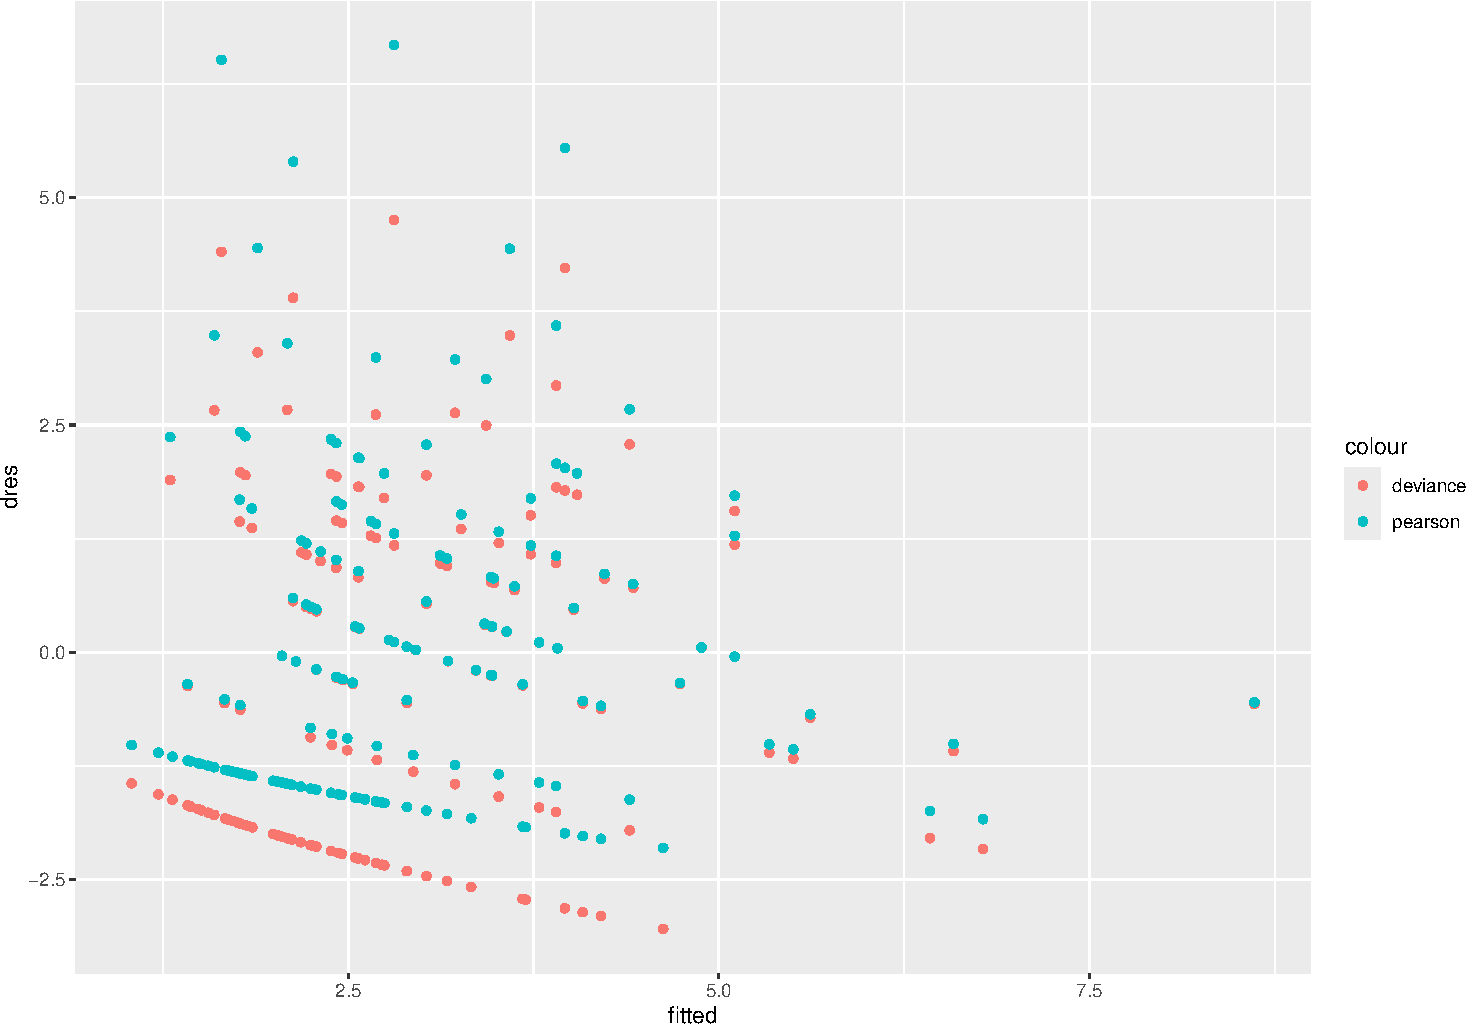
\includegraphics{Module04PoissonGammaPresentationWeek2_files/figure-beamer/unnamed-chunk-4-1.pdf}
\end{frame}

\begin{frame}[fragile]
\begin{block}{Pearson Residuals}
\protect\hypertarget{pearson-residuals-1}{}
\begin{Shaded}
\begin{Highlighting}[]
\NormalTok{gg2 }\OtherTok{=} \FunctionTok{ggplot}\NormalTok{(df) }\SpecialCharTok{+} \FunctionTok{geom\_point}\NormalTok{(}\FunctionTok{aes}\NormalTok{(}\AttributeTok{x =}\NormalTok{ fitted, }\AttributeTok{y =}\NormalTok{ pres, }\AttributeTok{color =}\NormalTok{ Sa))}
\NormalTok{gg2}
\end{Highlighting}
\end{Shaded}

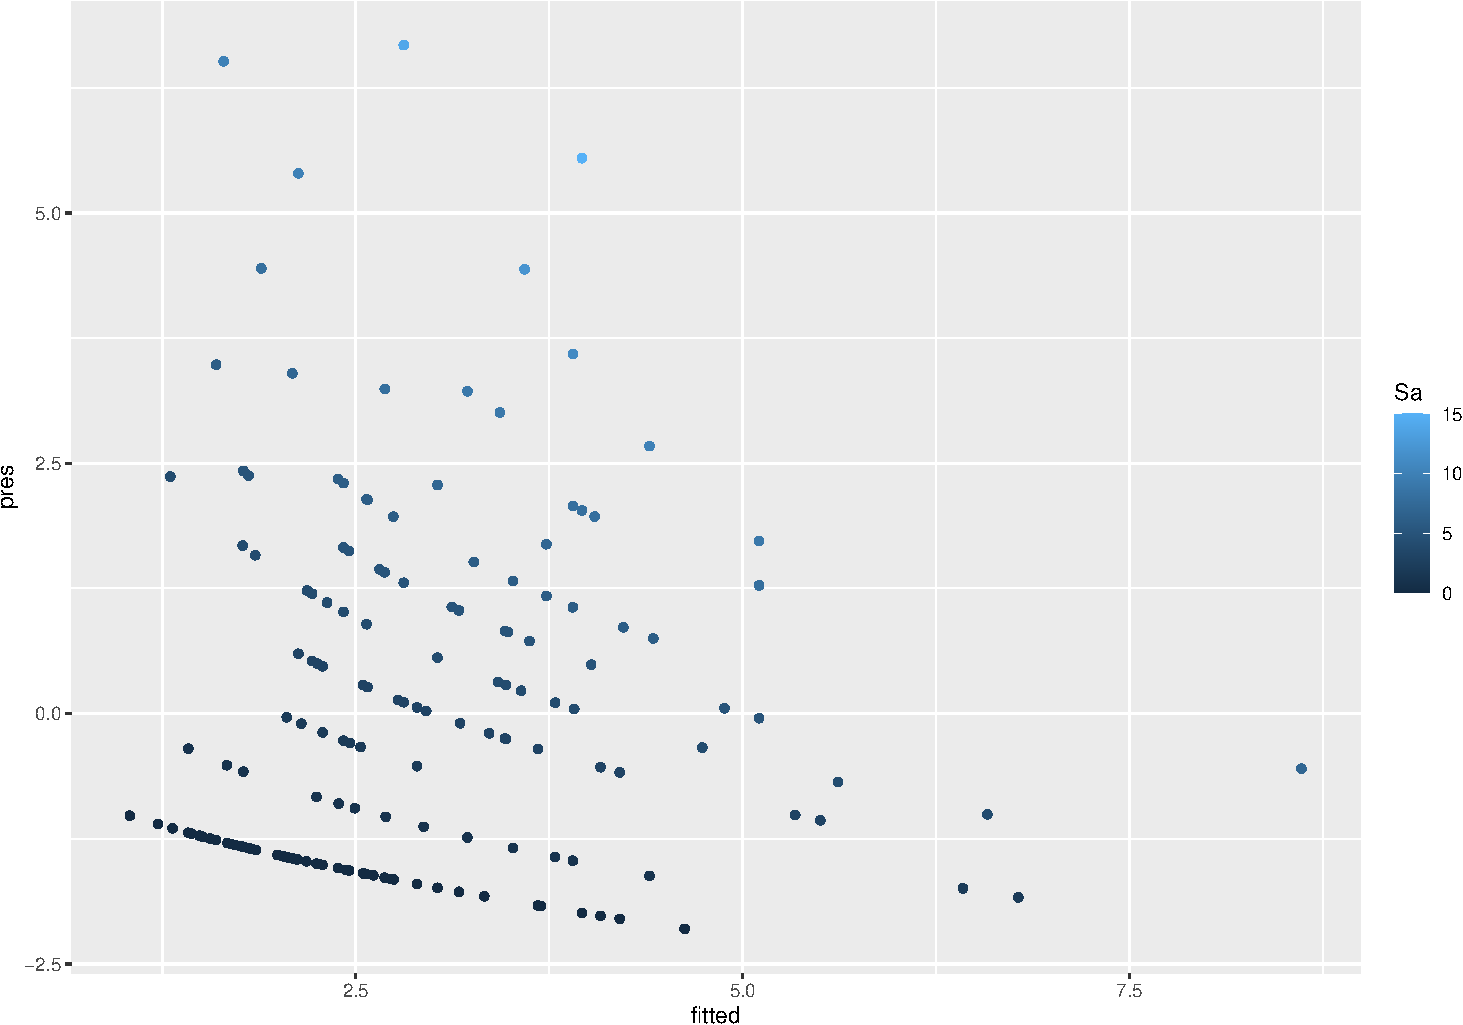
\includegraphics{Module04PoissonGammaPresentationWeek2_files/figure-beamer/unnamed-chunk-5-1.pdf}
\end{block}
\end{frame}

\begin{frame}[fragile]
\begin{block}{Normal Prabability Plots}
\protect\hypertarget{normal-prabability-plots}{}
\begin{Shaded}
\begin{Highlighting}[]
\NormalTok{dff }\OtherTok{=} \FunctionTok{data.frame}\NormalTok{(}\AttributeTok{devres =} \FunctionTok{residuals}\NormalTok{(model3, }\AttributeTok{type =} \StringTok{"deviance"}\NormalTok{), }\AttributeTok{pearsonres =} \FunctionTok{residuals}\NormalTok{(model3,}
    \AttributeTok{type =} \StringTok{"pearson"}\NormalTok{))}
\FunctionTok{ggplot}\NormalTok{(dff, }\FunctionTok{aes}\NormalTok{(}\AttributeTok{sample =}\NormalTok{ devres)) }\SpecialCharTok{+} \FunctionTok{stat\_qq}\NormalTok{(}\AttributeTok{pch =} \DecValTok{19}\NormalTok{) }\SpecialCharTok{+} \FunctionTok{geom\_abline}\NormalTok{(}\AttributeTok{intercept =} \DecValTok{0}\NormalTok{,}
    \AttributeTok{slope =} \DecValTok{1}\NormalTok{, }\AttributeTok{linetype =} \StringTok{"dotted"}\NormalTok{) }\SpecialCharTok{+} \FunctionTok{labs}\NormalTok{(}\AttributeTok{x =} \StringTok{"Theoretical quantiles"}\NormalTok{, }\AttributeTok{y =} \StringTok{"Deviance residuals"}\NormalTok{,}
    \AttributeTok{title =} \StringTok{"Normal Q{-}Q"}\NormalTok{, }\AttributeTok{subtitle =} \FunctionTok{deparse}\NormalTok{(model3}\SpecialCharTok{$}\NormalTok{call))}
\end{Highlighting}
\end{Shaded}

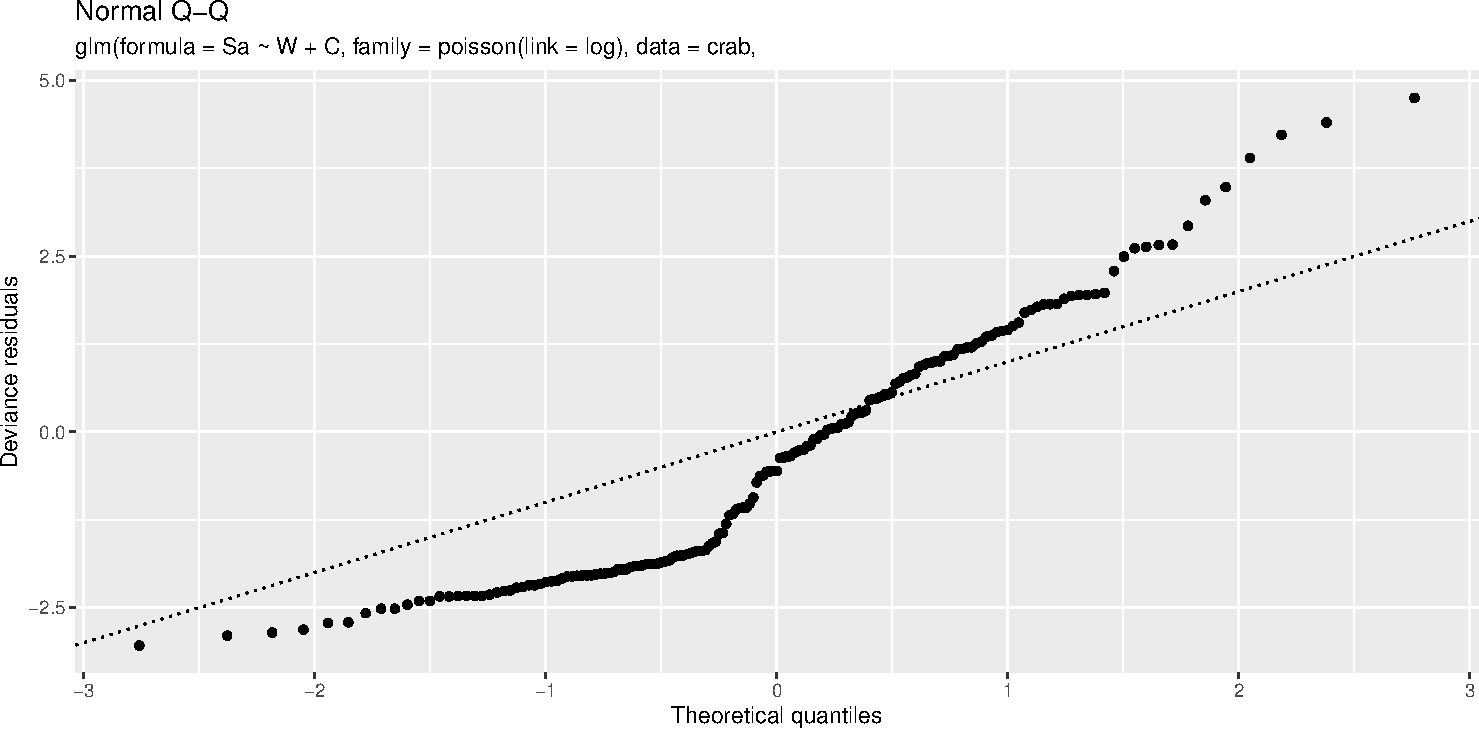
\includegraphics{Module04PoissonGammaPresentationWeek2_files/figure-beamer/unnamed-chunk-6-1.pdf}
\end{block}
\end{frame}

\begin{frame}[fragile]
\begin{Shaded}
\begin{Highlighting}[]
\FunctionTok{ggplot}\NormalTok{(dff, }\FunctionTok{aes}\NormalTok{(}\AttributeTok{sample =}\NormalTok{ pearsonres)) }\SpecialCharTok{+} \FunctionTok{stat\_qq}\NormalTok{(}\AttributeTok{pch =} \DecValTok{19}\NormalTok{) }\SpecialCharTok{+} \FunctionTok{geom\_abline}\NormalTok{(}\AttributeTok{intercept =} \DecValTok{0}\NormalTok{,}
    \AttributeTok{slope =} \DecValTok{1}\NormalTok{, }\AttributeTok{linetype =} \StringTok{"dotted"}\NormalTok{) }\SpecialCharTok{+} \FunctionTok{labs}\NormalTok{(}\AttributeTok{x =} \StringTok{"Theoretical quantiles"}\NormalTok{, }\AttributeTok{y =} \StringTok{"Pearson residuals"}\NormalTok{,}
    \AttributeTok{title =} \StringTok{"Normal Q{-}Q"}\NormalTok{, }\AttributeTok{subtitle =} \FunctionTok{deparse}\NormalTok{(model3}\SpecialCharTok{$}\NormalTok{call))}
\end{Highlighting}
\end{Shaded}

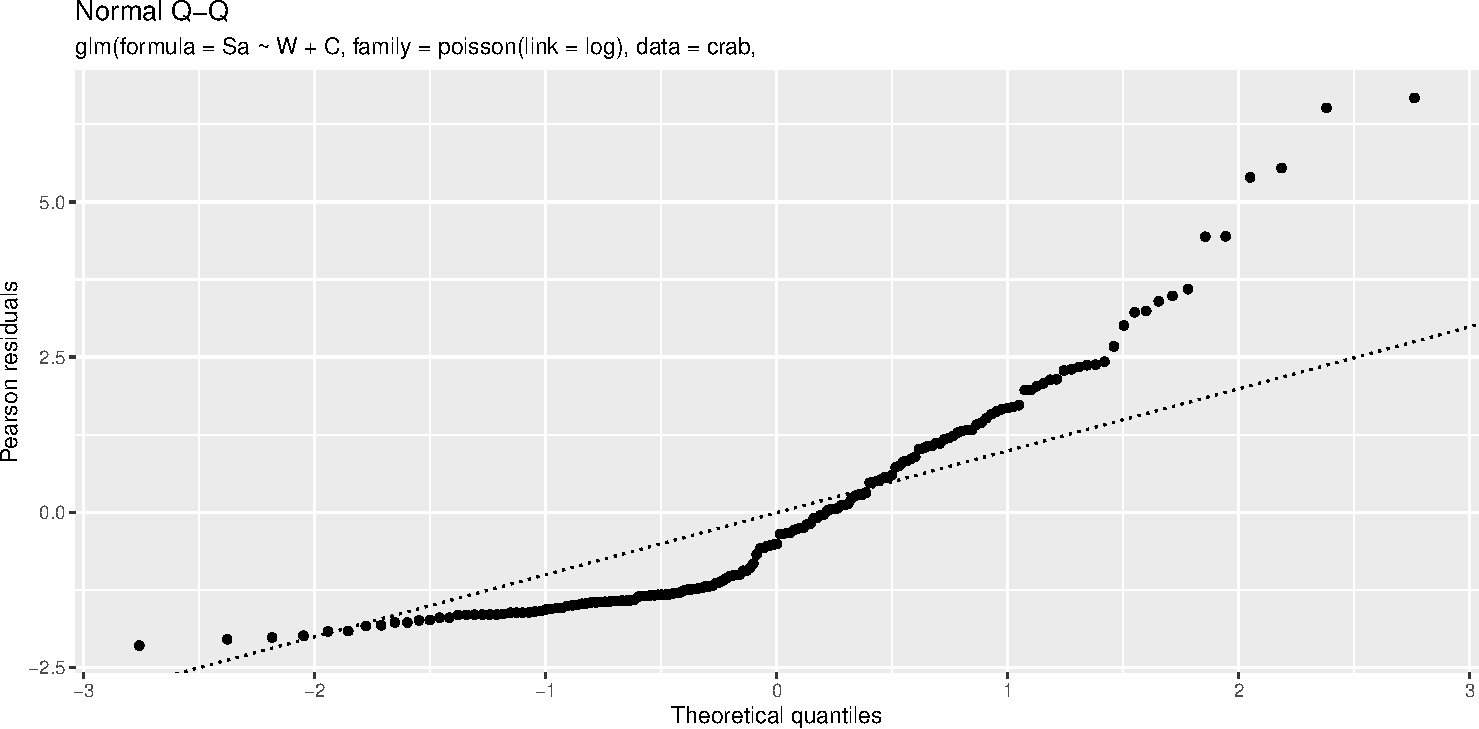
\includegraphics{Module04PoissonGammaPresentationWeek2_files/figure-beamer/unnamed-chunk-7-1.pdf}
\end{frame}

\begin{frame}{Overdispersion}
\protect\hypertarget{overdispersion}{}
Count data might show greater variability in the response counts than we
would expect if the response followed a Poisson distribution. This is
called \emph{overdispersion}.

Example: newspaper sales with tourist bus.

Our model states that the variance \(\text{Var}(Y_i)=\lambda_i\). If we
change the model to \(\text{Var}(Y_i)=\phi\lambda_i\) we may allow for
an increased variance due to heterogeneity among subjects.

Or, we can miss several covariate, then any daya point is a mixture of
several Poisson populations, each with its own mean for the response.

This heterogeniety may give an overall response distribution where the
variance is greater than the standard Poisson variance.
\end{frame}

\begin{frame}
The overdispersion parameter can be estimated from the Pearson statistic
or deviance

\[\hat{\phi}_D = \frac{1}{n-p} D\]

where \(D\) is the deviance. Note that similarity to
\(\hat{\sigma^2} = 1/(n-p)\cdot\text{SSE}\) in the MLR.

Cov\((\hat{\beta})\) can then be changed to
\(\hat{\phi}F^{-1}(\hat{\beta})\), so we multiply the standard error by
the square root of \(\hat{\phi}_D\).
\end{frame}

\begin{frame}[fragile]{Estimating Overdispersion}
\protect\hypertarget{estimating-overdispersion}{}
(more on quasipoisson later in the course)

\begin{Shaded}
\begin{Highlighting}[]
\NormalTok{model.od }\OtherTok{=} \FunctionTok{glm}\NormalTok{(Sa }\SpecialCharTok{\textasciitilde{}}\NormalTok{ W, }\AttributeTok{family =} \FunctionTok{poisson}\NormalTok{(}\AttributeTok{link =}\NormalTok{ log), }\AttributeTok{data =}\NormalTok{ crab)}
\NormalTok{model.disp }\OtherTok{=} \FunctionTok{glm}\NormalTok{(Sa }\SpecialCharTok{\textasciitilde{}}\NormalTok{ W, }\AttributeTok{family =} \FunctionTok{quasipoisson}\NormalTok{(}\AttributeTok{link =}\NormalTok{ log), }\AttributeTok{data =}\NormalTok{ crab)}
\CommentTok{\# summary.glm(model.od)}
\FunctionTok{summary.glm}\NormalTok{(model.disp)}\SpecialCharTok{$}\NormalTok{dispersion}

\NormalTok{(OverDisp.Dev }\OtherTok{\textless{}{-}}\NormalTok{ model.od}\SpecialCharTok{$}\NormalTok{deviance}\SpecialCharTok{/}\NormalTok{model.od}\SpecialCharTok{$}\NormalTok{df.residual)}
\NormalTok{Chi2 }\OtherTok{\textless{}{-}} \FunctionTok{sum}\NormalTok{((crab}\SpecialCharTok{$}\NormalTok{Sa }\SpecialCharTok{{-}} \FunctionTok{fitted}\NormalTok{(model.od))}\SpecialCharTok{\^{}}\DecValTok{2}\SpecialCharTok{/}\FunctionTok{fitted}\NormalTok{(model.od))}
\NormalTok{(OverDisp.Chi2 }\OtherTok{\textless{}{-}}\NormalTok{ Chi2}\SpecialCharTok{/}\NormalTok{model.od}\SpecialCharTok{$}\NormalTok{df.residual)}
\end{Highlighting}
\end{Shaded}

\begin{verbatim}
## [1] 3.182205
## [1] 3.320927
## [1] 3.182205
\end{verbatim}
\end{frame}

\begin{frame}{Rate models}
\protect\hypertarget{rate-models}{}
In the Poisson process we might analyse an event that occurs within a
time interval or region in space, and therefore it is often of interest
to model the \emph{rate} at which events occur.

Examples:

\begin{itemize}
\tightlist
\item
  crime rates in cities
\item
  death rate for smokers vs.~non-smokers
\item
  rate of auto thefts in cities
\end{itemize}

We model the rates by using an \emph{offset} to convert to counts.
\end{frame}

\begin{frame}
We don't want a model for \(Y_i\) but for \(Y_i/t_i\):

\begin{itemize}
\tightlist
\item
  Let \(t_i\) denote the index (population size in the example)
  associated with observation \(i\).
\item
  We still assume that \(Y_i\) follows a Poisson distribution, but we
  now include the index in the modelling and focus on \(Y_i/t_i\).
\item
  The expected value of \(Y_i/t_i\) would then be
  \(\text{E}(Y_i)/t_i=\lambda_i/t_i\).
\end{itemize}

A log-linear model would be \[ \log(\lambda_i/t_i)={\bf x}_i^T \beta\]
We may equivalently write the model as

\[
\log(\lambda_i)-\log(t_i)={\bf x}_i^T \beta
\] This adjustment term is called an \emph{offset} and is a known
quantity. Equivalently we have
\(\log(\lambda_i)={\bf x}_i^T \beta + \log(t_i)\)

The expected number of outcomes will then satisfy
\[ \text{E}(Y_i)=\lambda_i=t_i \exp({\bf x}_i^T \beta).\]
\end{frame}

\begin{frame}[fragile]
\begin{block}{Example: British doctors and rate models}
\protect\hypertarget{example-british-doctors-and-rate-models}{}
British doctors sent a questionnaire (in 1951) about whether they smoked
tobacco, and later information about their deaths were collected.

Research questions:

\begin{enumerate}
[1)]
\tightlist
\item
  Is the death rate higher for smokers than for non-smokers?
\item
  If so, by how much?
\item
  How is this related to age?
\end{enumerate}

\begin{Shaded}
\begin{Highlighting}[]
\FunctionTok{library}\NormalTok{(boot)}
\FunctionTok{data}\NormalTok{(breslow)}
\CommentTok{\# n=person{-}year, ns=smoker{-}years, y=number of deaths due to cad,}
\NormalTok{breslow}\SpecialCharTok{$}\NormalTok{age }\OtherTok{\textless{}{-}} \FunctionTok{factor}\NormalTok{(breslow}\SpecialCharTok{$}\NormalTok{age)  }\CommentTok{\#age=midpoint 10 year age group, }
\NormalTok{breslow}\SpecialCharTok{$}\NormalTok{smoke }\OtherTok{\textless{}{-}} \FunctionTok{factor}\NormalTok{(breslow}\SpecialCharTok{$}\NormalTok{smoke)  }\CommentTok{\# smoke=smoking status}
\end{Highlighting}
\end{Shaded}
\end{block}
\end{frame}

\begin{frame}[fragile]{Writing an offset}
\protect\hypertarget{writing-an-offset}{}
Here our count depends on \(n\)

(we are actually using a Poisson approximation to hte binomial)

There are 2 ways of coding an offset in \texttt{R}:

\begin{Shaded}
\begin{Highlighting}[]
\CommentTok{\# first age and smoke (but not interaction thereof)}
\NormalTok{fit1 }\OtherTok{\textless{}{-}} \FunctionTok{glm}\NormalTok{(y }\SpecialCharTok{\textasciitilde{}}\NormalTok{ age }\SpecialCharTok{+}\NormalTok{ smoke, }\AttributeTok{offset =} \FunctionTok{log}\NormalTok{(n), }\AttributeTok{family =}\NormalTok{ poisson, }\AttributeTok{data =}\NormalTok{ breslow)}
\NormalTok{fit1a }\OtherTok{\textless{}{-}} \FunctionTok{glm}\NormalTok{(y }\SpecialCharTok{\textasciitilde{}}\NormalTok{ age }\SpecialCharTok{+}\NormalTok{ smoke }\SpecialCharTok{+} \FunctionTok{offset}\NormalTok{(}\FunctionTok{log}\NormalTok{(n)), }\AttributeTok{family =}\NormalTok{ poisson, }\AttributeTok{data =}\NormalTok{ breslow)}
\end{Highlighting}
\end{Shaded}
\end{frame}

\begin{frame}[fragile]{Do we need an interaction?}
\protect\hypertarget{do-we-need-an-interaction}{}
\begin{Shaded}
\begin{Highlighting}[]
\CommentTok{\# do we need interaction?}
\NormalTok{fit2 }\OtherTok{\textless{}{-}} \FunctionTok{update}\NormalTok{(fit1, . }\SpecialCharTok{\textasciitilde{}}\NormalTok{ . }\SpecialCharTok{+}\NormalTok{ smoke }\SpecialCharTok{*}\NormalTok{ age)}
\FunctionTok{anova}\NormalTok{(fit1, fit2, }\AttributeTok{test =} \StringTok{"Chisq"}\NormalTok{)}
\end{Highlighting}
\end{Shaded}

\begin{verbatim}
## Analysis of Deviance Table
## 
## Model 1: y ~ age + smoke
## Model 2: y ~ age + smoke + age:smoke
##   Resid. Df Resid. Dev Df Deviance Pr(>Chi)  
## 1         4     12.132                       
## 2         0      0.000  4   12.132  0.01639 *
## ---
## Signif. codes:  0 '***' 0.001 '**' 0.01 '*' 0.05 '.' 0.1 ' ' 1
\end{verbatim}
\end{frame}

\begin{frame}[fragile]{The final model}
\protect\hypertarget{the-final-model}{}
Number of deaths per 1000 doctors.

\begin{Shaded}
\begin{Highlighting}[]
\CommentTok{\# year 40 nonsmokers should only be the intercept}
\FunctionTok{exp}\NormalTok{(fit2}\SpecialCharTok{$}\NormalTok{coefficients[}\DecValTok{1}\NormalTok{]) }\SpecialCharTok{*} \DecValTok{1000}
\CommentTok{\# 80 year olds who smoke}
\DecValTok{1000} \SpecialCharTok{*} \FunctionTok{exp}\NormalTok{(}\FunctionTok{sum}\NormalTok{(fit2}\SpecialCharTok{$}\NormalTok{coefficients[}\FunctionTok{c}\NormalTok{(}\DecValTok{1}\NormalTok{, }\DecValTok{5}\NormalTok{, }\DecValTok{6}\NormalTok{, }\DecValTok{10}\NormalTok{)]))}
\end{Highlighting}
\end{Shaded}

\begin{verbatim}
## (Intercept) 
##   0.1064396 
## [1] 19.18375
\end{verbatim}

(you can also use \texttt{predict()} to do this)
\end{frame}

\begin{frame}{Modelling continuous positive response data}
\protect\hypertarget{modelling-continuous-positive-response-data}{}
\begin{block}{Examples of continuous positive responses}
\protect\hypertarget{examples-of-continuous-positive-responses}{}
\begin{itemize}
\tightlist
\item
  Insurance: Claim sizes
\item
  Medicine: Time to blood coagulation (main example)
\item
  Biology: Time in various development stages for fruit fly
\item
  Meteorology: Amount of precipitation (interactive session - exam
  question 2012)
\end{itemize}

This is also covered in \textbf{survival analysis}, but that often
sidesteps modelling the actual distributions
\end{block}
\end{frame}

\begin{frame}
\begin{block}{Models for continuous positive responses}
\protect\hypertarget{models-for-continuous-positive-responses}{}
\begin{itemize}
\tightlist
\item
  Lognormal distribution on response
\item
  Gamma distribution on response
\item
  Inverse Gaussian distribution on response (we will not consider this
  here)
\end{itemize}
\end{block}
\end{frame}

\begin{frame}[fragile]
\begin{block}{Time to blood coagulation}
\protect\hypertarget{time-to-blood-coagulation}{}
The data is clotting time of blood (in seconds) \texttt{y} for normal
plasma diluted to nine different percentage concentrations \texttt{u}
with prothrombin-free plasma (whatever that is!).

To induce the clotting a chemical called thromboplasting was used, and
in the experiment two different lots of the chemical were used - denoted
\texttt{lot}. Our aim is to investigate the relationship between the
clotting time and the dilution percentage, and look at differences
between the lots.
\end{block}
\end{frame}

\begin{frame}[fragile]
\begin{Shaded}
\begin{Highlighting}[]
\NormalTok{clot }\OtherTok{=} \FunctionTok{read.table}\NormalTok{(}\StringTok{"https://www.math.ntnu.no/emner/TMA4315/2018h/clot.txt"}\NormalTok{, }\AttributeTok{header =}\NormalTok{ T)}
\NormalTok{clot}\SpecialCharTok{$}\NormalTok{lot }\OtherTok{=} \FunctionTok{as.factor}\NormalTok{(clot}\SpecialCharTok{$}\NormalTok{lot)}
\FunctionTok{summary}\NormalTok{(clot)}
\end{Highlighting}
\end{Shaded}

\begin{verbatim}
##        u            time       lot  
##  Min.   :  5   Min.   : 12.0   1:9  
##  1st Qu.: 15   1st Qu.: 18.0   2:9  
##  Median : 30   Median : 23.0        
##  Mean   : 40   Mean   : 32.5        
##  3rd Qu.: 60   3rd Qu.: 35.0        
##  Max.   :100   Max.   :118.0
\end{verbatim}
\end{frame}

\begin{frame}{Lognormal distribution}
\protect\hypertarget{lognormal-distribution}{}
Let \(Y_i\) be the response on the original scale, where \(Y_i>0\).

Transform the response to a logaritmic scale: \(Y^*_i=\ln(Y_i)\). Then,
assume that transformed responses follow a normal distribution (or
follows approximately) and use ordinary MLR. This means we have a GLM
with normal response and identity link (on logarithmic scale of
reponse).

\begin{enumerate}
\tightlist
\item
  \(Y^*_i \sim N(\mu^{*}_i,\sigma^{*2})\)
\item
  \(\eta_i={\bf x}_i^T\beta\)
\item
  \(\mu^{*}_i=\eta_i\) (identity link)
\end{enumerate}
\end{frame}

\begin{frame}
There are two ways of looking at this,

\begin{enumerate}
\tightlist
\item
  either this is just a transformation to achieve approximate normality,
  or
\item
  we assume that the original data follows a lognormal distribution.
\end{enumerate}

In genomics one usually assume the former, and reports back results on
the exponential scale - just say that the mean of original data is
\(\exp(\mu^{*}_i)\).

However, if on instead assume that the original data really comes from a
lognormal distribution, then it can be shown that

\[\text{E}(Y_i)=\exp(\mu^{*}_i) \cdot \exp(\sigma^{*2}/2)\]
\[\text{Var}(Y_i) =\exp(\sigma^{*2} -1)\cdot \mu_i^2\]

i.e.~standard deviation proportional to expectation.
\end{frame}

\begin{frame}{Gamma regression}
\protect\hypertarget{gamma-regression}{}
\begin{block}{The gamma distribution}
\protect\hypertarget{the-gamma-distribution}{}
We have seen that a gamma distributed variable may be the result of the
time between events in a Poisson process. The well known
\(\chi^2_{\delta}\)-distribution is a special case of the gamma
distribution (\(\frac{\nu}{\mu_i}=2\), \(\nu=\frac{\delta}{2}\)).

There are many parameterization for the gamma distribution, but we will
stick with the one used in our textbook (page 643):

\(Y_i \sim Ga(\mu_i,\nu)\) with density
\[ f(y_i)=\frac{1}{\Gamma(\nu)} (\frac{\nu}{\mu_i})^{\nu} y_i^{\nu-1}\exp(-\frac{\nu}{\mu_i}y_i) \text{ for }y_i>0\]
\end{block}
\end{frame}

\begin{frame}[fragile]{Comparing the lognormal and gamma}
\protect\hypertarget{comparing-the-lognormal-and-gamma}{}
\begin{Shaded}
\begin{Highlighting}[]
\NormalTok{orgmu }\OtherTok{=} \DecValTok{1}
\NormalTok{orgsd }\OtherTok{=} \FloatTok{0.3}  \CommentTok{\# normal mean and sd}
\NormalTok{mu }\OtherTok{=} \FunctionTok{exp}\NormalTok{(orgmu }\SpecialCharTok{+}\NormalTok{ orgsd}\SpecialCharTok{\^{}}\DecValTok{2}\SpecialCharTok{/}\DecValTok{2}\NormalTok{)  }\CommentTok{\# = shape*scale}
\NormalTok{scale }\OtherTok{=}\NormalTok{ (}\FunctionTok{exp}\NormalTok{(orgsd}\SpecialCharTok{\^{}}\DecValTok{2}\NormalTok{) }\SpecialCharTok{{-}} \DecValTok{1}\NormalTok{) }\SpecialCharTok{*}\NormalTok{ mu}
\NormalTok{shape }\OtherTok{=}\NormalTok{ mu}\SpecialCharTok{/}\NormalTok{scale}
\FunctionTok{library}\NormalTok{(ggplot2)}
\NormalTok{xrange }\OtherTok{=} \FunctionTok{range}\NormalTok{(}\DecValTok{0}\NormalTok{, }\DecValTok{10}\NormalTok{)}
\end{Highlighting}
\end{Shaded}
\end{frame}

\begin{frame}[fragile]{These should have the same mean and variance}
\protect\hypertarget{these-should-have-the-same-mean-and-variance}{}
\begin{Shaded}
\begin{Highlighting}[]
\FunctionTok{ggplot}\NormalTok{(}\FunctionTok{data.frame}\NormalTok{(}\AttributeTok{x =}\NormalTok{ xrange), }\FunctionTok{aes}\NormalTok{(xrange)) }\SpecialCharTok{+} \FunctionTok{xlab}\NormalTok{(}\FunctionTok{expression}\NormalTok{(x)) }\SpecialCharTok{+} \FunctionTok{stat\_function}\NormalTok{(}\AttributeTok{fun =}\NormalTok{ dlnorm,}
    \AttributeTok{args =} \FunctionTok{list}\NormalTok{(}\AttributeTok{meanlog =}\NormalTok{ orgmu, }\AttributeTok{sdlog =}\NormalTok{ orgsd), }\AttributeTok{geom =} \StringTok{"line"}\NormalTok{, }\AttributeTok{colour =} \StringTok{"red"}\NormalTok{, }\AttributeTok{n =} \DecValTok{1001}\NormalTok{) }\SpecialCharTok{+}
    \FunctionTok{stat\_function}\NormalTok{(}\AttributeTok{fun =}\NormalTok{ dgamma, }\AttributeTok{args =} \FunctionTok{list}\NormalTok{(}\AttributeTok{shape =}\NormalTok{ shape, }\AttributeTok{scale =}\NormalTok{ scale), }\AttributeTok{geom =} \StringTok{"line"}\NormalTok{,}
        \AttributeTok{colour =} \StringTok{"blue"}\NormalTok{)}
\end{Highlighting}
\end{Shaded}

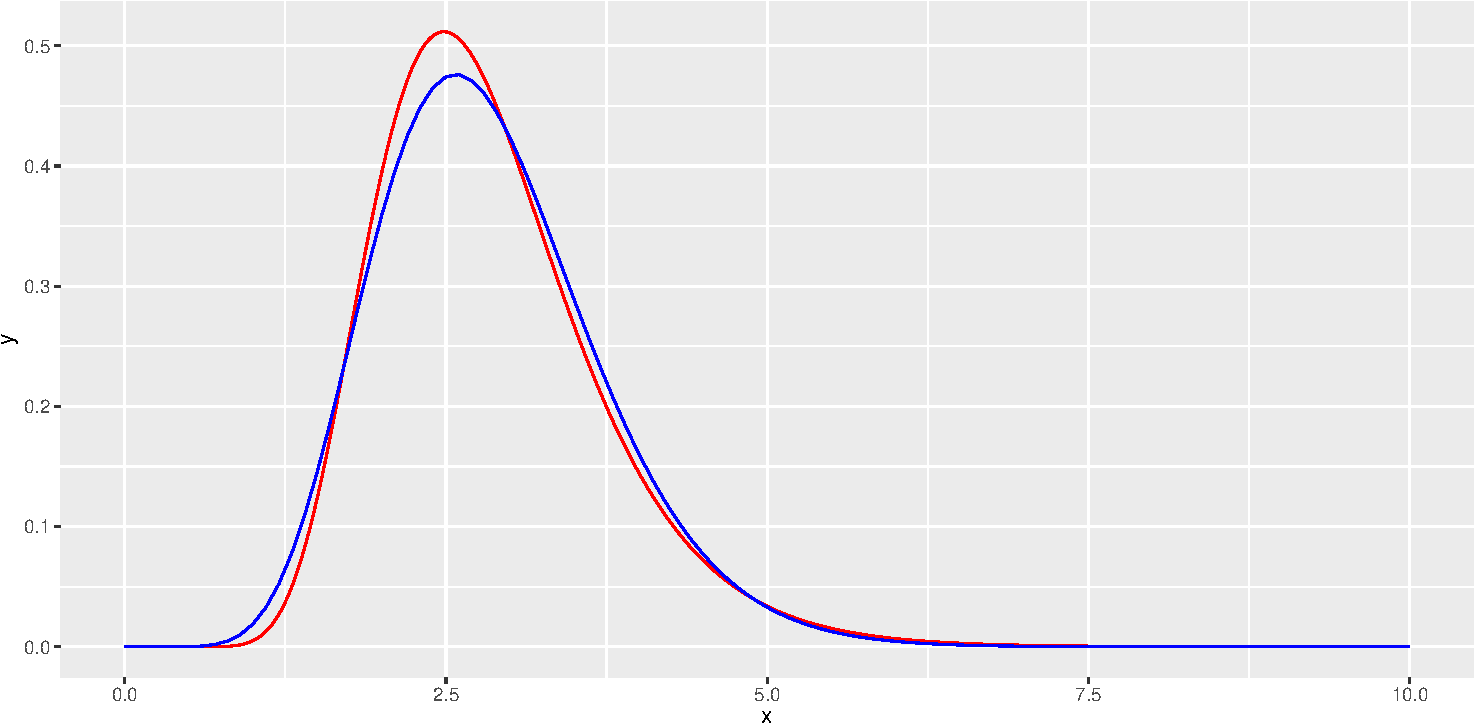
\includegraphics{Module04PoissonGammaPresentationWeek2_files/figure-beamer/unnamed-chunk-15-1.pdf}
\end{frame}

\begin{frame}
We found in Module 1 that the gamma distribution is an exponential
family, with

\begin{itemize}
\tightlist
\item
  \(\theta_i=-\frac{1}{\mu_i}\) is the canonical parameter
\item
  \(\phi=\frac{1}{\nu}\),
\item
  \(w_i=1\)
\item
  \(b(\theta_i)=-\ln(-\theta_i)\)
\item
  \(\text{E}(Y_i)=b'(\theta_i)=-\frac{1}{\theta_i}=\mu_i\)
\item
  \(\text{Var}(Y_i)=b''(\theta_i)\frac{\psi}{w_i}=\frac{\mu_i^2}{\nu}\)
\end{itemize}

(if you don't remember, work it out!)
\end{frame}

\begin{frame}
For a GLM model we have canonical link if \[\theta_i=\eta_i\] Since
\(\eta_i=g(\mu_i)\) this means to us that we need
\[\theta_i=g(\mu_i)=-\frac{1}{\mu_i}\] saying that with the canonical
link is \(-\frac{1}{\mu_i}\).

However, the most commonly used link is \(g(\mu_i)=\ln(\mu_i)\), and the
identity link is also used.

\textbf{Q:} Discuss the implications on \(\eta_i\) when using the
canonical link. Why might the log-link be preferred?
\end{frame}

\begin{frame}
Remark: often the inverse and not the negative inverse is used, and
since \[g(\mu_i)=-\frac{1}{\mu_i}={\bf x}_i^T\beta\] then
\[\frac{1}{\mu_i}=-{\bf x}_i^T\beta={\bf x}_i^T\beta^*\] where
\(\beta^*=-\beta\).
\end{frame}

\begin{frame}
\begin{block}{Gamma GLM model}
\protect\hypertarget{gamma-glm-model}{}
\begin{enumerate}
\item
  \(Y_i \sim Ga(\mu_i,\nu)\)
\item
  \(\eta_i={\bf x}_i^T\beta\)
\item
  Popular link functions:

  \begin{itemize}
  \tightlist
  \item
    \(\eta_i=\mu_i\) (identity link)
  \item
    \(\eta_i=\frac{1}{\mu_i}\) (inverse link)
  \item
    \(\eta_i=\ln(\mu_i)\) (log-link)
  \end{itemize}
\end{enumerate}

\textbf{Remark:} In our model the parameter \(\mu_i\) varies with \(i\)
but \(\nu\) is the same for all observations.
\end{block}
\end{frame}

\begin{frame}[fragile]
\begin{block}{Example: Time to blood coagulation}
\protect\hypertarget{example-time-to-blood-coagulation}{}
A simple model to start with is as follows (dosages often analysed on
log scale):

\tiny

\begin{Shaded}
\begin{Highlighting}[]
\NormalTok{fit1 }\OtherTok{=} \FunctionTok{glm}\NormalTok{(time }\SpecialCharTok{\textasciitilde{}}\NormalTok{ lot }\SpecialCharTok{+} \FunctionTok{log}\NormalTok{(u), }\AttributeTok{data =}\NormalTok{ clot, }\AttributeTok{family =} \FunctionTok{Gamma}\NormalTok{(}\AttributeTok{link =}\NormalTok{ log))}
\FunctionTok{summary}\NormalTok{(fit1)}
\end{Highlighting}
\end{Shaded}

\begin{verbatim}
## 
## Call:
## glm(formula = time ~ lot + log(u), family = Gamma(link = log), 
##     data = clot)
## 
## Coefficients:
##             Estimate Std. Error t value Pr(>|t|)    
## (Intercept)  5.44660    0.13453   40.48  < 2e-16 ***
## lot2        -0.47034    0.07095   -6.63 8.02e-06 ***
## log(u)      -0.58476    0.03772  -15.50 1.22e-10 ***
## ---
## Signif. codes:  0 '***' 0.001 '**' 0.01 '*' 0.05 '.' 0.1 ' ' 1
## 
## (Dispersion parameter for Gamma family taken to be 0.02265072)
## 
##     Null deviance: 7.7087  on 17  degrees of freedom
## Residual deviance: 0.3211  on 15  degrees of freedom
## AIC: 104.28
## 
## Number of Fisher Scoring iterations: 5
\end{verbatim}

\normalsize

\textbf{Q}: describe what you see in the print-out.
\end{block}
\end{frame}

\begin{frame}{Gamma regression: likelihood and derivations thereof}
\protect\hypertarget{gamma-regression-likelihood-and-derivations-thereof}{}
\textbf{Likelihood:}
\[L(\beta)=\prod_{i=1}^n \exp(-\frac{\nu y_i}{\mu_i}-\nu \ln \mu_i +\nu \ln \nu +(\nu-1)\ln y_i -\ln(\Gamma(\nu)))\]

\textbf{Log-likelihood:}
\[l(\beta)=\sum_{i=1}^n [-\frac{\nu y_i}{\mu_i}-\nu \ln \mu_i +\nu \ln \nu +(\nu-1)\ln y_i -\ln(\Gamma(\nu))]\]
Observe that we now- for the first time - have a nuisance parameter
\(\nu\) here.
\end{frame}

\begin{frame}{Fitting the Model}
\protect\hypertarget{fitting-the-model}{}
To produce numerical estimates for the parameter of interest \(\beta\)
we may proceed to the score function, and solve using Newton Raphson or
Fisher scoring. If we do not have the canonical link the observed and
expected Fisher information matrix may not be equal.

What about \(\phi=1/\nu\)? Also estimated using maximum likelihood.

Further analyses: as before we use asymptotic distribution of parameter
estimates, and of Wald, LRT and score test.
\end{frame}

\begin{frame}[fragile]{Scaled and unscaled deviance}
\protect\hypertarget{scaled-and-unscaled-deviance}{}
We have defined the deviance as
\[D=-2(\ln L(\text{candidate model})-\ln L(\text{saturated model}))\]

This is often called the \emph{scaled deviance}.

The \emph{unscaled deviance} is then defined as \(\phi D\), but is sadly
sometimes also called the deviance - for example by \texttt{R}.

\begin{enumerate}
\item
  For the normal model the

  \begin{itemize}
  \tightlist
  \item
    scaled deviance is
    \(D=\frac{1}{\sigma^2}\sum_{i=1}^n (y_i-\hat{\mu}_i)^2\), while
  \item
    unscaled deviance is \(\phi D=\sum_{i=1}^n (y_i-\hat{\mu}_i)^2\)
  \end{itemize}
\item
  For the binomial and Poisson model \(\phi=1\) so the scaled and
  unscaled deviance are equal.
\item
  What about the Gamma model?
\end{enumerate}
\end{frame}

\begin{frame}[fragile]
Some calculations - see IL week 2, problem 2: 1b.

\[D=\frac{-2 \sum_{i=1}^n [\ln (\frac{y_i}{\hat{\mu}_i})-\frac{y_i-\hat{\mu}_i}{\hat{\mu}_i}]}{\phi}\]
and unscaled as
\(\phi D=-2 \sum_{i=1}^n [\ln (\frac{y_i}{\hat{\mu}_i})-\frac{y_i-\hat{\mu}_i}{\hat{\mu}_i}]\).

Compare to print-out from R: the deviance in R is the \emph{unscaled
deviance}.

\begin{Shaded}
\begin{Highlighting}[]
\FunctionTok{deviance}\NormalTok{(fit1)}
\NormalTok{(}\AttributeTok{nu1 =} \DecValTok{1}\SpecialCharTok{/}\FunctionTok{summary}\NormalTok{(fit1)}\SpecialCharTok{$}\NormalTok{dispersion)}
\NormalTok{(}\AttributeTok{D =} \SpecialCharTok{{-}}\DecValTok{2} \SpecialCharTok{*}\NormalTok{ nu1 }\SpecialCharTok{*} \FunctionTok{sum}\NormalTok{(}\FunctionTok{log}\NormalTok{(fit1}\SpecialCharTok{$}\NormalTok{y}\SpecialCharTok{/}\NormalTok{fit1}\SpecialCharTok{$}\NormalTok{fitted.values) }\SpecialCharTok{{-}}\NormalTok{ ((fit1}\SpecialCharTok{$}\NormalTok{y }\SpecialCharTok{{-}}\NormalTok{ fit1}\SpecialCharTok{$}\NormalTok{fitted.values)}\SpecialCharTok{/}\NormalTok{fit1}\SpecialCharTok{$}\NormalTok{fitted.values)))}
\FunctionTok{deviance}\NormalTok{(fit1) }\SpecialCharTok{*}\NormalTok{ nu1}
\end{Highlighting}
\end{Shaded}

\begin{verbatim}
## [1] 0.3210963
## [1] 44.14871
## [1] 14.17599
## [1] 14.17599
\end{verbatim}
\end{frame}

\begin{frame}[fragile]{Comparing models}
\protect\hypertarget{comparing-models}{}
\begin{block}{Comparing models based on deviance}
\protect\hypertarget{comparing-models-based-on-deviance}{}
\begin{Shaded}
\begin{Highlighting}[]
\NormalTok{fit2 }\OtherTok{=} \FunctionTok{glm}\NormalTok{(time }\SpecialCharTok{\textasciitilde{}}\NormalTok{ lot }\SpecialCharTok{+} \FunctionTok{log}\NormalTok{(u) }\SpecialCharTok{+}\NormalTok{ lot}\SpecialCharTok{:}\FunctionTok{log}\NormalTok{(u), }\AttributeTok{data =}\NormalTok{ clot, }\AttributeTok{family =} \FunctionTok{Gamma}\NormalTok{(}\AttributeTok{link =}\NormalTok{ log))}
\FunctionTok{anova}\NormalTok{(fit1, fit2)}
\end{Highlighting}
\end{Shaded}

\begin{verbatim}
## Analysis of Deviance Table
## 
## Model 1: time ~ lot + log(u)
## Model 2: time ~ lot + log(u) + lot:log(u)
##   Resid. Df Resid. Dev Df  Deviance
## 1        15    0.32110             
## 2        14    0.31576  1 0.0053352
\end{verbatim}

The deviance table does not include \(\phi\), so the unscaled deviance
is reported. If significance testing is done, the estimated \(\phi\)
from the largest model is used, and \(p\)-values are based on the scaled
deviance.
\end{block}
\end{frame}

\begin{frame}[fragile]
\begin{Shaded}
\begin{Highlighting}[]
\FunctionTok{anova}\NormalTok{(fit1, fit2, }\AttributeTok{test =} \StringTok{"Chisq"}\NormalTok{)}
\DecValTok{1} \SpecialCharTok{{-}} \FunctionTok{pchisq}\NormalTok{((}\FunctionTok{deviance}\NormalTok{(fit1) }\SpecialCharTok{{-}} \FunctionTok{deviance}\NormalTok{(fit2))}\SpecialCharTok{/}\FunctionTok{summary}\NormalTok{(fit2)}\SpecialCharTok{$}\NormalTok{dispersion, fit1}\SpecialCharTok{$}\NormalTok{df.residual }\SpecialCharTok{{-}}
\NormalTok{    fit2}\SpecialCharTok{$}\NormalTok{df.residual)}
\FunctionTok{anova}\NormalTok{(fit1, fit2, }\AttributeTok{test =} \StringTok{"F"}\NormalTok{)}
\DecValTok{1} \SpecialCharTok{{-}} \FunctionTok{pf}\NormalTok{((}\FunctionTok{deviance}\NormalTok{(fit1) }\SpecialCharTok{{-}} \FunctionTok{deviance}\NormalTok{(fit2))}\SpecialCharTok{/}\FunctionTok{summary}\NormalTok{(fit2)}\SpecialCharTok{$}\NormalTok{dispersion, fit1}\SpecialCharTok{$}\NormalTok{df.residual }\SpecialCharTok{{-}}
\NormalTok{    fit2}\SpecialCharTok{$}\NormalTok{df.residual, fit2}\SpecialCharTok{$}\NormalTok{df.residual)}
\end{Highlighting}
\end{Shaded}

\begin{verbatim}
## Analysis of Deviance Table
## 
## Model 1: time ~ lot + log(u)
## Model 2: time ~ lot + log(u) + lot:log(u)
##   Resid. Df Resid. Dev Df  Deviance Pr(>Chi)
## 1        15    0.32110                      
## 2        14    0.31576  1 0.0053352   0.6355
## [1] 0.6355477
## Analysis of Deviance Table
## 
## Model 1: time ~ lot + log(u)
## Model 2: time ~ lot + log(u) + lot:log(u)
##   Resid. Df Resid. Dev Df  Deviance      F Pr(>F)
## 1        15    0.32110                           
## 2        14    0.31576  1 0.0053352 0.2246 0.6429
## [1] 0.642854
\end{verbatim}
\end{frame}

\begin{frame}[fragile]
\begin{block}{Comparing models based on AIC}
\protect\hypertarget{comparing-models-based-on-aic}{}
\begin{Shaded}
\begin{Highlighting}[]
\FunctionTok{AIC}\NormalTok{(fit1, fit2)}
\end{Highlighting}
\end{Shaded}

\begin{verbatim}
##      df      AIC
## fit1  4 104.2763
## fit2  5 105.9738
\end{verbatim}

\textbf{Q}: would you prefer \texttt{fit1} or \texttt{fit2}?
\end{block}
\end{frame}

\begin{frame}
AIC can also be used when we compare models with different link
functions (models that are not nested).

The literature suggests to plot \(y_i\) vs.~each covariate to get a hint
about which link function or transformation to use.

\begin{itemize}
\tightlist
\item
  Identity: Plot of \(y_i\) vs \(x_i\) should be close to linear
\item
  \(\ln:\) Plot of \(\ln(y_i)\) vs \(x_i\) should be close to linear
\item
  Inverse (reciprocal): Plot of \(1/y_i\) vs \(x_i\) should be close to
  linear
\end{itemize}
\end{frame}

\begin{frame}[fragile]{Compare link functions}
\protect\hypertarget{compare-link-functions}{}
\begin{Shaded}
\begin{Highlighting}[]
\FunctionTok{library}\NormalTok{(ggplot2)}
\FunctionTok{library}\NormalTok{(ggpubr)}
\NormalTok{y }\OtherTok{=}\NormalTok{ clot}\SpecialCharTok{$}\NormalTok{time}
\NormalTok{x }\OtherTok{=}\NormalTok{ clot}\SpecialCharTok{$}\NormalTok{u}

\NormalTok{df }\OtherTok{=} \FunctionTok{data.frame}\NormalTok{(}\AttributeTok{y =}\NormalTok{ y, }\AttributeTok{x =}\NormalTok{ x)}
\NormalTok{gg1 }\OtherTok{=} \FunctionTok{ggplot}\NormalTok{(df) }\SpecialCharTok{+} \FunctionTok{geom\_point}\NormalTok{(}\FunctionTok{aes}\NormalTok{(}\AttributeTok{x =} \FunctionTok{log}\NormalTok{(x), }\AttributeTok{y =}\NormalTok{ y)) }\SpecialCharTok{+} \FunctionTok{ggtitle}\NormalTok{(}\StringTok{"Identity"}\NormalTok{)}
\NormalTok{gg2 }\OtherTok{=} \FunctionTok{ggplot}\NormalTok{(df) }\SpecialCharTok{+} \FunctionTok{geom\_point}\NormalTok{(}\FunctionTok{aes}\NormalTok{(}\AttributeTok{x =} \FunctionTok{log}\NormalTok{(x), }\AttributeTok{y =} \FunctionTok{log}\NormalTok{(y))) }\SpecialCharTok{+} \FunctionTok{ggtitle}\NormalTok{(}\StringTok{"Log"}\NormalTok{)}
\NormalTok{gg3 }\OtherTok{=} \FunctionTok{ggplot}\NormalTok{(df) }\SpecialCharTok{+} \FunctionTok{geom\_point}\NormalTok{(}\FunctionTok{aes}\NormalTok{(}\AttributeTok{x =} \FunctionTok{log}\NormalTok{(x), }\AttributeTok{y =} \DecValTok{1}\SpecialCharTok{/}\NormalTok{y)) }\SpecialCharTok{+} \FunctionTok{ggtitle}\NormalTok{(}\StringTok{"Inverse"}\NormalTok{)}
\NormalTok{gg4 }\OtherTok{=} \FunctionTok{ggplot}\NormalTok{(df) }\SpecialCharTok{+} \FunctionTok{geom\_point}\NormalTok{(}\FunctionTok{aes}\NormalTok{(}\AttributeTok{x =} \FunctionTok{sqrt}\NormalTok{(}\DecValTok{1}\SpecialCharTok{/}\NormalTok{x), }\AttributeTok{y =} \FunctionTok{log}\NormalTok{(y))) }\SpecialCharTok{+} \FunctionTok{ggtitle}\NormalTok{(}\StringTok{"Log, sqrt x"}\NormalTok{)}
\end{Highlighting}
\end{Shaded}
\end{frame}

\begin{frame}[fragile]
\begin{Shaded}
\begin{Highlighting}[]
\FunctionTok{ggarrange}\NormalTok{(gg1, gg2, gg3, gg4)}
\end{Highlighting}
\end{Shaded}

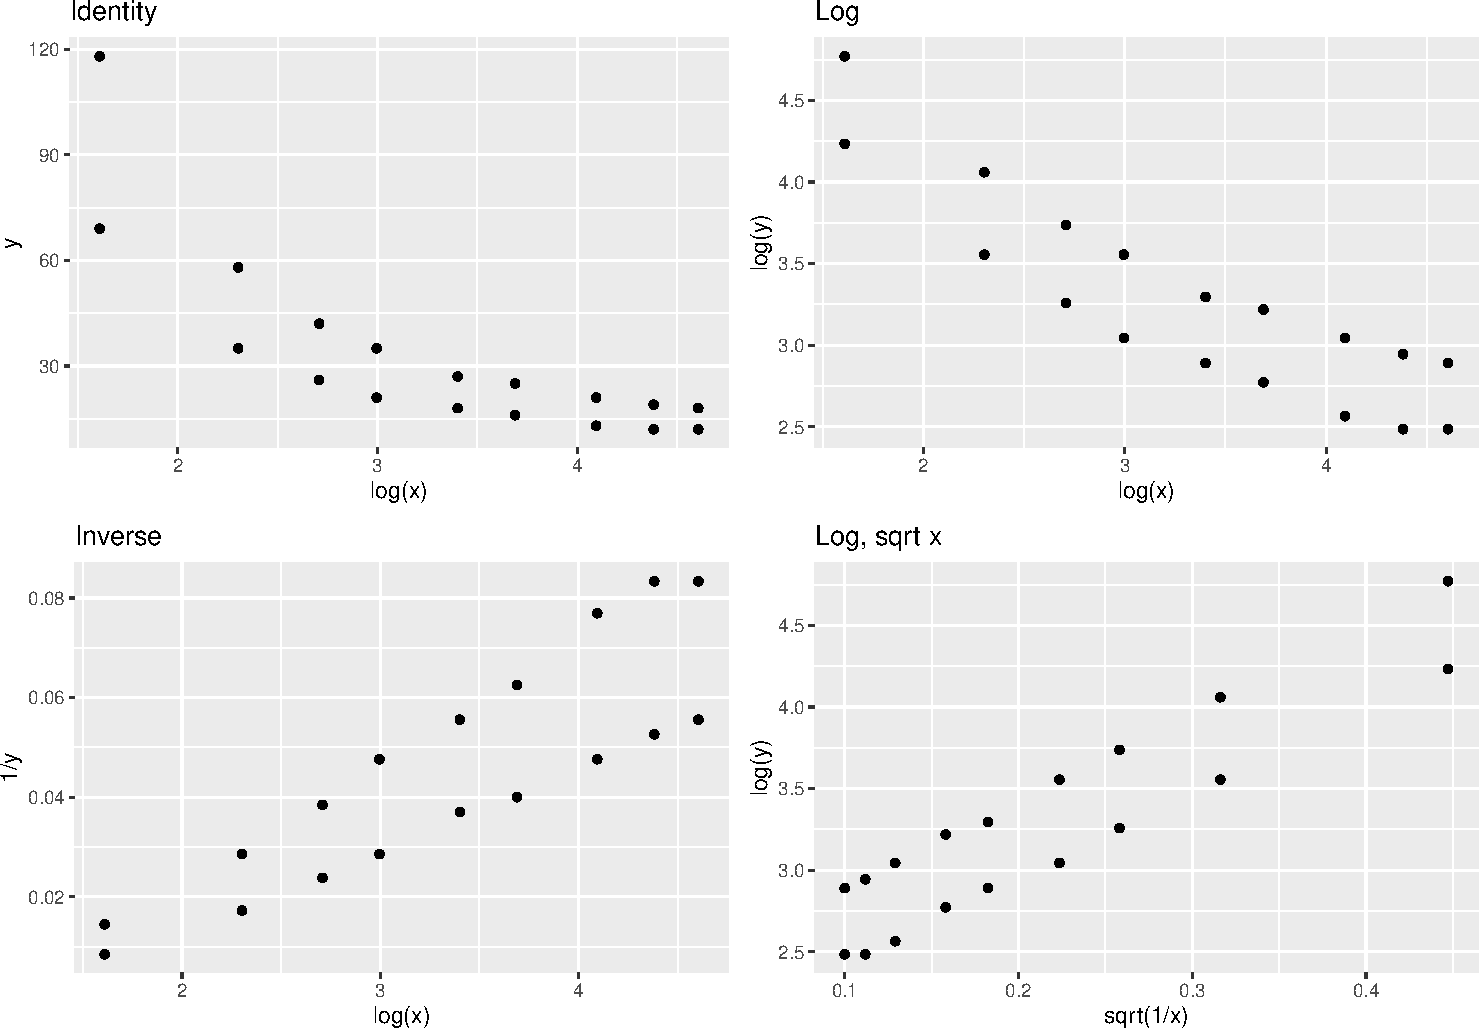
\includegraphics{Module04PoissonGammaPresentationWeek2_files/figure-beamer/unnamed-chunk-22-1.pdf}
\end{frame}

\begin{frame}[fragile]
\begin{Shaded}
\begin{Highlighting}[]
\NormalTok{fit4 }\OtherTok{=} \FunctionTok{glm}\NormalTok{(time }\SpecialCharTok{\textasciitilde{}}\NormalTok{ lot }\SpecialCharTok{+} \FunctionTok{sqrt}\NormalTok{(}\DecValTok{1}\SpecialCharTok{/}\NormalTok{u), }\AttributeTok{data =}\NormalTok{ clot, }\AttributeTok{family =} \FunctionTok{Gamma}\NormalTok{(}\AttributeTok{link =}\NormalTok{ log))}
\FunctionTok{AIC}\NormalTok{(fit1, fit4)}
\end{Highlighting}
\end{Shaded}

\begin{verbatim}
##      df       AIC
## fit1  4 104.27633
## fit4  4  45.01688
\end{verbatim}
\end{frame}

\begin{frame}[fragile]{Code for Residual Plots}
\protect\hypertarget{code-for-residual-plots}{}
\begin{Shaded}
\begin{Highlighting}[]
\NormalTok{df4 }\OtherTok{=} \FunctionTok{data.frame}\NormalTok{(}\AttributeTok{fitted =}\NormalTok{ fit4}\SpecialCharTok{$}\NormalTok{fitted.values, }\AttributeTok{dres =} \FunctionTok{residuals}\NormalTok{(fit4, }\AttributeTok{type =} \StringTok{"deviance"}\NormalTok{))}
\NormalTok{gg4 }\OtherTok{=} \FunctionTok{ggplot}\NormalTok{(df4) }\SpecialCharTok{+} \FunctionTok{geom\_point}\NormalTok{(}\FunctionTok{aes}\NormalTok{(}\AttributeTok{x =}\NormalTok{ fitted, }\AttributeTok{y =}\NormalTok{ dres)) }\SpecialCharTok{+} \FunctionTok{scale\_color\_discrete}\NormalTok{(}\StringTok{""}\NormalTok{) }\SpecialCharTok{+}
    \FunctionTok{ggtitle}\NormalTok{(}\StringTok{"time\textasciitilde{}lot+sqrt(1/u)"}\NormalTok{)}
\NormalTok{df1 }\OtherTok{=} \FunctionTok{data.frame}\NormalTok{(}\AttributeTok{fitted =}\NormalTok{ fit1}\SpecialCharTok{$}\NormalTok{fitted.values, }\AttributeTok{dres =} \FunctionTok{residuals}\NormalTok{(fit1, }\AttributeTok{type =} \StringTok{"deviance"}\NormalTok{))}
\NormalTok{gg1 }\OtherTok{=} \FunctionTok{ggplot}\NormalTok{(df1) }\SpecialCharTok{+} \FunctionTok{geom\_point}\NormalTok{(}\FunctionTok{aes}\NormalTok{(}\AttributeTok{x =}\NormalTok{ fitted, }\AttributeTok{y =}\NormalTok{ dres)) }\SpecialCharTok{+} \FunctionTok{scale\_color\_discrete}\NormalTok{(}\StringTok{""}\NormalTok{) }\SpecialCharTok{+}
    \FunctionTok{ggtitle}\NormalTok{(}\StringTok{"time\textasciitilde{}lot+log(u)"}\NormalTok{)}
\end{Highlighting}
\end{Shaded}
\end{frame}

\begin{frame}[fragile]{The Plots}
\protect\hypertarget{the-plots}{}
Are these good?

\begin{Shaded}
\begin{Highlighting}[]
\FunctionTok{ggarrange}\NormalTok{(gg1, gg4)}
\end{Highlighting}
\end{Shaded}

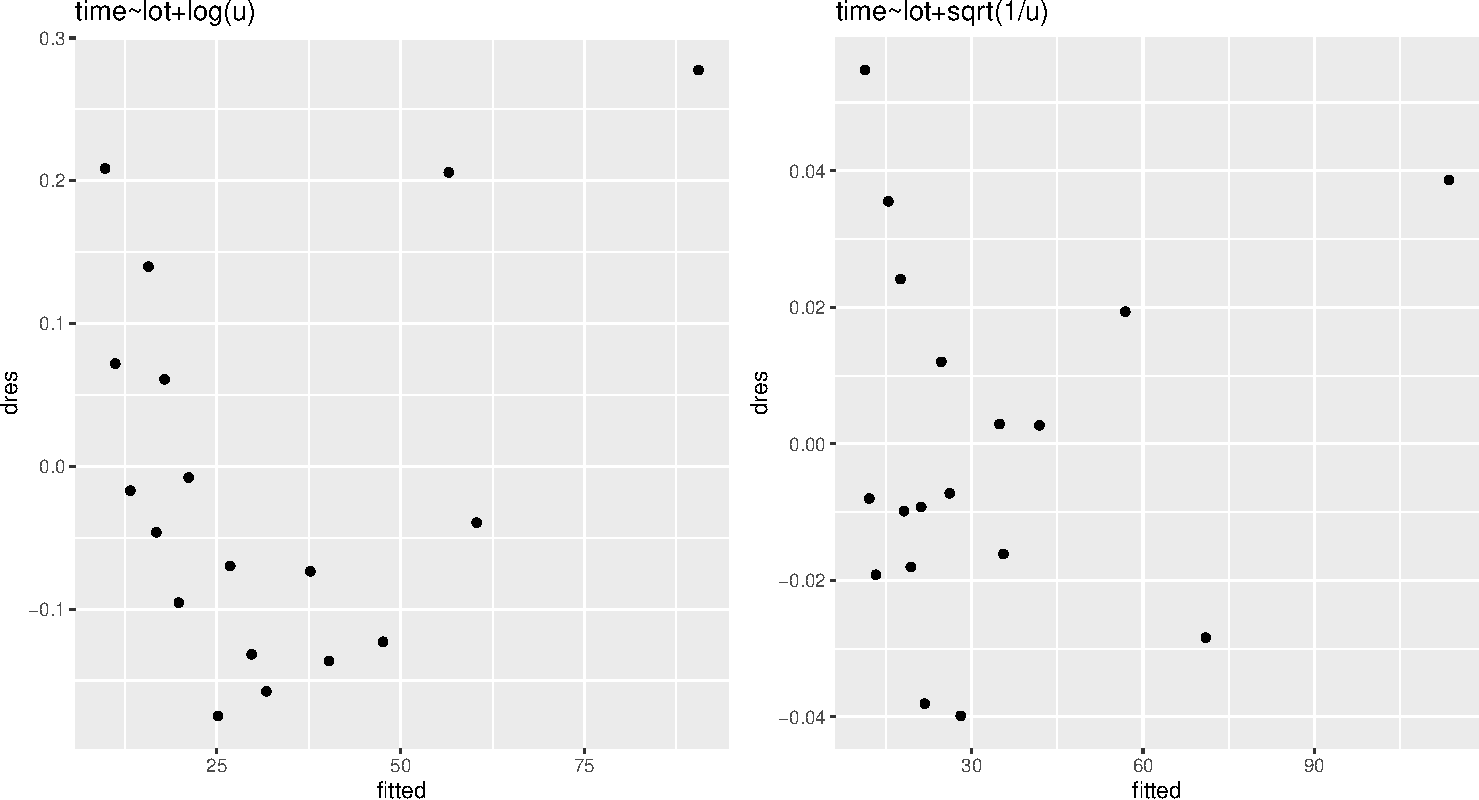
\includegraphics{Module04PoissonGammaPresentationWeek2_files/figure-beamer/unnamed-chunk-25-1.pdf}
\end{frame}

\begin{frame}[fragile]{R packages}
\protect\hypertarget{r-packages}{}
\begin{Shaded}
\begin{Highlighting}[]
\FunctionTok{install.packages}\NormalTok{(}\FunctionTok{c}\NormalTok{(}\StringTok{"tidyverse"}\NormalTok{, }\StringTok{"ggplot2"}\NormalTok{, }\StringTok{"statmod"}\NormalTok{, }\StringTok{"corrplot"}\NormalTok{, }\StringTok{"ggplot2"}\NormalTok{, }\StringTok{"GGally"}\NormalTok{,}
    \StringTok{"boot"}\NormalTok{))}
\end{Highlighting}
\end{Shaded}
\end{frame}

\begin{frame}{Further reading}
\protect\hypertarget{further-reading}{}
\begin{itemize}
\tightlist
\item
  A. Agresti (1996): ``An Introduction to Categorical Data Analysis''.
\item
  A. Agresti (2015): ``Foundations of Linear and Generalized Linear
  Models.'' Wiley.
\item
  A. J. Dobson and A. G. Barnett (2008): ``An Introduction to
  Generalized Linear Models'', Third edition.
\item
  J. Faraway (2015): ``Extending the Linear Model with R'', Second
  Edition. \url{http://www.maths.bath.ac.uk/~jjf23/ELM/}
\item
  P. McCullagh and J. A. Nelder (1989): ``Generalized Linear Models''.
  Second edition.
\end{itemize}
\end{frame}

\end{document}
